\section{Theorie}
Um Röntgenstrahlen zu erzeugen werden aus einer Glühkathode
Elektronen emittiert und zur Anode hin beschleunigt. Beim Auftreffen auf die
Anode entsteht eine Röntgenstrahlung. Diese setzt sich aus dem 
kontiniuerlichen Bremsspektrum und der charakteristischen Röntgenstrahlung
des Anodenmaterials zusammen.
Bei der Abbremsung eines Elektrons im Coulombfeld des
Atomkerns entsteht das Bremsspektrum, das zum kontiniuerlichen Spektrum gezählt wird, da
ein Photon ausgesendet wird und dessen Energie gleich dem Energieverlust des abgebremsten
Elektrons ist. Bei vollständiger Abbremsung wird die maximale Energie und somit die 
minimale Wellenlänge erreicht
\begin{align}
\lambda_{\text{min}} &= \frac{h \cdot c}{e_0U} \,.
\end{align}
Dabei ist $h$ das Planck´sche Wirkungsquantum, $c$ die Lichtgeschwindikeit, $e_0$ die Elementarladung
und $U$ die Spannung.
Es wird die gesamte kinetische Energie
\begin{align*}
    E_{\text{kin}} &= e_0U
\end{align*}
in Strahlungsenergie 
\begin{align*}
    E &= hv 
\end{align*}
umgewandelt, wobei $v$ die Frequenz ist. In Abbildung \ref{fig:kontiSpektrum1}
ist die Wellenlänge gegen die Intensität aufgetragen.
\begin{figure}[H]
    \centering
    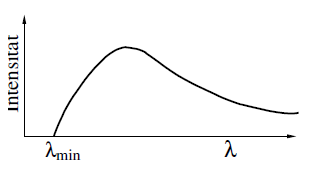
\includegraphics{kontiSpektrum.png}
    \caption{Das kontiniuerliche Bremsspektrum-Die Intensität in Abhängigkeit der Wellenlänge \protect\cite{AL}.} 
    \label{fig:kontiSpektrum1}
\end{figure}Beim charakteristischen Spektrum wird das Anodenmaterial ionisiert.
Dabei entsteht eine Leerstelle in einer inneren Schale, sodass ein Elektron
aus einer äußeren Schale unter Aussendung eines Röntgenquants in diese 
Leerstelle zurückfällt. Die Energie des Photons ist dann die Energiedifferenz der
beiden Energieniveaus
\begin{align}
    h \nu &= E_m - E_n \,.
\end{align}
Das Spektrum besteht folglich aus scharfen Linien, die mit 
$K_\alpha$, $K_\beta$, $L_\alpha$ usw. bezeichnet werden.
Die Großbuchstaben stehen für die Schalen, auf denen die Übergänge enden. Die griechischen Buchstaben geben an, woher die beteiligten äußeren Elektronen stammen.
\begin{figure}[H]
    \centering
    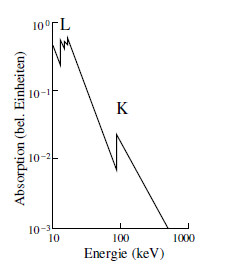
\includegraphics{Graphik.png}
    \caption{Der Photoabsorptionskoeffizient in Abhängigkeit von der Photonenenergie,welche, je nach Schale aus der das Elektron stammt, als K-, L-,M- Absorptionskante bezeichnet wird\protect\cite{AL}.}
    \label{fig:kontiSpektrum}
\end{figure}
Bei den Mehrelektronenatomen schirmen die Hüllenelektronen und die Wechselwirkungen der Elektronen die
Kernladung ab, somit verringert sich die Coulomb-Anziehung auf das äußere
Elektron. Die Bindungsenergie ist dann
\begin{align}
    E_n &= -R_\infty z_{\text{eff}}^2 \cdot \frac{1}{n^2}
\end{align}
mit der effektiven Kernladung 
\begin{align*}
    z_{\text{eff}} &= z - \sigma,
\end{align*}
die Abschirmkonstante $\sigma$ und die Rydbergkonstante $R_\infty = 13,6 \ \text{eV}$.
Daraus ergibt sich für die $K_\alpha$-Linie eine Abschirmkonstante
von
\begin{align}
    \sigma_{K_{\alpha}} &= R_\infty (z-\sigma_1)^2 \cdot \frac{1}{1^2} - R_\infty (z-\sigma_2)^2 \cdot \frac{1}{2^2} \,.
\end{align}
Die Abschirmkonstante ist für jedes Elektron unterschiedlich und empirisch bestimmbar.
Die äußeren Elektronen besitzen wegen des Bahndrehimpulses und des Elektronenspins
nicht alle die selbe Bindungsenergie, daher liegen die charakteristischen Linien eng nebeneinander,
was als Feinstruktur bekannt ist. Dies kann im Versuch nicht aufgespalten
werden, daher werden Kupferanoden verwendet, bei denen Cu-$K_\alpha$- und Cu-$K_\beta$ - Linien
gesehen werden. Der Comptoneffekt und der Photoeffekt treten häufig bei der Absorption von Röntgenstahlung
unter 1 MeV auf. Es ist eine Abnahme des Absorptionskoeffzienten mit zunehmender
Energie zu erkennen. Dieser steigt jedoch auch sprunghaft an, wenn die Photonenenergie
größer als die Bindungsenergie ist. Die Bindungsenergie und die Absorptionskanten sind
fast identisch
\begin{align}
    h \nu_{\text{abs}} &= E_n - E_\infty \,.
\end{align}
Unter Berücksichtigung der Feinstruktur ergibt sich die Bindungsenergie: die
Sommerfeldsche Feinstruktur
\begin{align}
    E_{n,j} &= -R_\infty \left(z_{\text{eff},1}^2 \cdot \frac{1}{n^2} + \alpha^2 z_{\text{eff},2}^4 \cdot \left(\frac{1}{j+\frac{1}{2}} - \frac{3}{4n}\right)\right)
\end{align}
mit der Sommerfeldschen Feinstrukturkonstante $\alpha$, der Hauptquantenzahl n und dem
Gesamtdrehimpuls j. Mit Hilfe der Gleichungen (4) und (6) ergibt sich die Abschirmkonstante
der K-Kante zu
\begin{align}
    \sigma_K &= Z - \sqrt{\frac{E_K}{R_\infty} - \frac{\alpha^2 Z^4}{4}} \,.
\end{align}
Die Abschrimkonstante $\sigma_L$ kann mit Hilfe der Energiedifferenz $\Delta E$
zweier L-Kanten bestimmt werden. Es ergibt sich
\begin{align}
    \sigma_L &= Z - \left(\frac{4}{\alpha} \sqrt{\frac{\Delta E_L}{R_\infty}}-\frac{5 \Delta E_L}{R_\infty}\right)^{1/2} \left(1+\frac{19}{32} \alpha^2 \frac{\Delta E_L}{R_\infty}\right)^{1/2}
\end{align}
mit der Ordnungszahl Z.
Über die Braggsche Refexion wird die Energie bzw. Wellenlänge experimentell bestimmt.
In Abbildung \ref{fig:Bragg1} ist eine Skizze dazu. Das Röntgenlicht fällt auf ein 3 dimensionales
Gitter, zum Beispiel ein LiF-Kristall. Dabei wird das Photon an jedem Atom des
Gitters gebeugt. Beim Glanzwinkel $\theta$ entsteht konstruktive Interferenz. Die Bragg'sche
Bedingung lautet
\begin{align}
    \text{2d} \sin (\theta) &= \text{n} \lambda
\end{align}
mit der Gitterkonstante d ($d_{\text{LiF}}=201,4 \ \text{pm}$) und der Beugungsordnung n.
\begin{figure}[H]
    \centering
    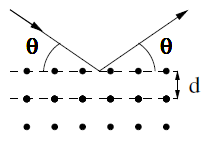
\includegraphics{Bragg1.png}
    \caption{Bragg´sche Reflexion- Die Energie $E$ bzw die Wellenlänge $\lambda$ der Röntgenstrahlung durch die Bragg’sche Reflexion. Die Röntgenbeugung am dreidimensionalen Gitter mit dem Bragg-Winkel\protect\cite{AL}.}
    \label{fig:Bragg1}
\end{figure}


\label{sec:Theorie}

